\documentclass[12pt]{article}
\usepackage[margin=0.75in]{geometry}
\usepackage{multicol}
\usepackage[fleqn]{amsmath}
\usepackage{mathtools}
\usepackage{array}
\usepackage{tabularx}
\usepackage{tcolorbox}
\usepackage{xcolor}
\usepackage{amssymb}
\usepackage{amsthm}
\usepackage{lastpage}
\usepackage{fancyhdr}
\usepackage{setspace}
\usepackage{hyperref}
\mathindent=0.0pt
\onehalfspacing
\AtBeginDocument{
  \addtolength\abovedisplayskip{-0.5\baselineskip}
  \addtolength\belowdisplayskip{-0.5\baselineskip}
}
\pagestyle{fancy}
\setlength{\headheight}{15pt}
\setlength{\columnsep}{2cm}
\graphicspath{{./Images/}}

%%%%%Setting tag color for mark tags&&&&&
\newtagform{red}{\color{red}[}{]}
\usetagform{red}
\newcommand{\ansgiven}{\tag{A.G.}}
\newcommand{\ansmark}{\tag{A1}}
\newcommand{\onemark}{\tag{M1}}
\newcommand{\twomark}{\tag{M2}}
\newcommand{\qnmark}[1]{\hfill \text[#1]}

%%%%%Black square QED symbol%%%%%
\renewcommand{\qedsymbol}{\ensuremath{\blacksquare}}

%%%%%Hyperref Setup%%%%%
\hypersetup{
  colorlinks=true,
  linkcolor=blue,
  filecolor=magenta,
  urlcolor=cyan,
} % add packages, settings, and declarations in Preamble.tex

\title{FurtherQ \\* Problem Set 1}
\author{Public Edition \\* Version 2.0}
\date{October 2022}


\begin{document}

\maketitle
%%%%%Table of Contents%%%%%

\textbf{\\\Large{Problems}}\\
\textit{
  \large
  \hyperlink{P1}{Problem 1} \dotfill 2\\*
  \hyperlink{P2}{Problem 2} \dotfill 3\\*
  \hyperlink{P3}{Problem 3} \dotfill 4\\*
  \hyperlink{P4}{Problem 4} \dotfill 6\\*
  \hyperlink{P5}{Problem 5} \dotfill 8\\*
  \hyperlink{P6}{Problem 6} \dotfill 10\\*
  \hyperlink{P7}{Problem 7} \dotfill 15\\*
  \hyperlink{P8}{Problem 8} \dotfill 18\\*
  \hyperlink{P9}{Problem 9} \dotfill 21\\*
  \hyperlink{P10}{Problem 10} \dotfill 23\\
}

\begin{multicols*}{2}
      \textbf{\Large{Editions}} \\
      \textit{
          \hspace*{13.5pt} PB - Public Edition \\
          \hspace*{13.5pt} SS - Secondary School Edition \\
  }

      \textbf{\Large{Question Difficulty}} \\
      \textit{
            \hspace*{13.5pt} Easy - Warm up \\
            \hspace*{13.5pt} Intermediate - Standard \\
            \hspace*{13.5pt} Challenging - Difficult \\
            \hspace*{13.5pt} Schadenfreude - Interesting \\
            \hspace*{13.5pt} Extensions - Out of syllabus
  }

  \vspace*{40pt}

  \textit{This work is licensed under a \href{http://creativecommons.org/licenses/by/4.0/}{Creative \\ \hspace*{13.5pt} Commons Attribution 4.0 International \\ \hspace*{13.5pt} License}}

  \textbf{\Large{Organizing Team}} \\
  \textit{
        \hspace*{13pt} (Problem Setter) NousernameSG \\
        \hspace*{13pt} (Problem Setter) GrassGlass \\
        \hspace*{13pt} (Problem Vetter) Mr Cheng \\
  }

  \textbf{\Large{Paper Info}} \\
  \textit{
        \hspace*{13pt} Total Time: 180 Mins (3 hrs) \\
        \hspace*{13pt} Graded Questions: 1-8\(\;\,\&\;\)10 \\
        \hspace*{13pt} Total Marks: 105
  }
        \vspace*{15pt}

        \begin{tabularx}{0.37\textwidth} {
          | >{\centering\arraybackslash}X
          | >{\centering\arraybackslash}X | }
          \hline
          Attempted & \phantom{9}/9 \\
          \hline
          Grade & \\
          \hline
          Marks & \phantom{105}/105 \\
          \hline
          Percentage & \phantom{100}\% \\
          \hline
      \end{tabularx}
\end{multicols*}


\newpage

\lhead{FurtherQ - Problem Set 1}
\rhead{PB Edition - Version 2.0}

\cfoot{\thepage\ of \pageref{LastPage}}

%%%%%Problem Files%%%%%
\begin{enumerate}
  \item \textbf{\hypertarget{P1}{[\,Suggested Time: 7 mins \textbar \, Total Marks: 7 \textbar \, Easy\,]}}\\
    \textit{
        A function f is defined by \(\displaystyle f(x) = \sqrt{2}\left(\sin{x} + \cos{x} + 1\right)\) for \(0\le x\le 2\pi\)\\
        Points P and Q are the maximum and minimum points of f respectively,\\
        Without the use of calculus, find the coordinates P and Q \\
        \textbf{Leave your answers in exact values.}} \qnmark{7}

%%%%%%%%%%%%%%%%%%
%%%%%Solution%%%%%
%%%%%%%%%%%%%%%%%%

%\begin{comment}

%%%%%Combining sin x and cos x with R-Formula%%%%%
\begin{gather*}
    \displaystyle Let \; y = \sqrt{2}\sin{x} + \sqrt{2}\cos{x} + \sqrt{2} \\
    \displaystyle Let \; R\sin{(x + \alpha)} = \sqrt{2}\sin{x} + \sqrt{2}\cos{x} \onemark
\end{gather*}
\begin{align*}
    \displaystyle R\sin{\alpha} &= \sqrt{2} \\
    \displaystyle R\cos{\alpha} &= \sqrt{2}
\end{align*}
\begin{align*} %% Value of R
    \displaystyle R &= \sqrt{2+2} \\
                    &= 2 \onemark
\end{align*}
\begin{align*} %% Value of \alpha
    \displaystyle \alpha &= \tan^{-1}{(1)} \\
                         &= \frac{\pi}{4} \onemark
\end{align*}

%%%%%Rewriting the equation and finding P & Q%%%%%
\begin{gather*} %% Rewriting expression
    \displaystyle \implies\sqrt{2}\sin{x} + \sqrt{2}\cos{x} = 2\sin{\left(x + \frac{\pi}{4}\right)}\\
    \displaystyle \therefore y = 2\sin{\left(x + \frac{\pi}{4}\right)} + \sqrt{2}
\end{gather*}
\begin{multicols}{2}
    \begin{align*} %% Coordinate of P
        max(y) = 2 + \sqrt{2} \onemark \\
        when \; \sin{\left(x + \frac{\pi}{4}\right)} &= 1 \\
        \therefore x + \frac{\pi}{4} &= \frac{\pi}{2}\\
        x &= \frac{\pi}{4}
    \end{align*}
    \begin{equation*}
        \implies P = \left(\frac{\pi}{4} , 2 + \sqrt{2}\right) \ansmark
    \end{equation*}

    \begin{align*} %% Coordinate of Q
        min(y) = \sqrt{2} - 2 \onemark \\
        when \; \sin{\left(x + \frac{\pi}{4}\right)} &= -1\\
        \therefore x + \frac{\pi}{4} &= \frac{3\pi}{2}\\
        x &= \frac{5\pi}{4}
    \end{align*}
    \begin{equation*}
        \implies Q = \left(\frac{5\pi}{4} , \sqrt{2} - 2\right) \ansmark
    \end{equation*}
\end{multicols}

%\end{comment} \newpage
  \item \textbf{\hypertarget{P2}{[\,Suggested Time: 5 mins \textbar \, Total Marks: 5 \textbar \, Easy\,]}}\\
    \textbf{Without the use of a calculator}, Solve the following equation \\
    \(\textstyle 6^{2x}+36^{x} = 2\sqrt[3]{\textstyle 6\sqrt[3]{\textstyle 216\sqrt[3]{6}}}\) \\
    Hence find the value of \(\displaystyle \sqrt[19]{\displaystyle 2^{6x}}\) \qnmark{5}

%%%%%%%%%%%%%%%%%%
%%%%%Solution%%%%%
%%%%%%%%%%%%%%%%%%

%\begin{comment}

%%%%%Finding the value of x%%%%%
\begin{align*}
    \displaystyle        6^{2x}+6^{2x} &= 2\left(6\left(6^{3}\left(6\right)^{\textstyle \frac{1}{3}}\right)^{\textstyle \frac{1}{3}}\right)^{\textstyle \frac{1}{3}} \\
    \displaystyle 2\left(6^{2x}\right) &= 2\left(6\left(6^{\textstyle \frac{10}{3}}\right)^{\textstyle \frac{1}{3}}\right)^{\textstyle \frac{1}{3}} \wrkonemark \\
    \displaystyle                      &= 2\left(6^{\textstyle 1+\frac{10}{9}}\right)^{\textstyle \frac{1}{3}} \\
    \displaystyle                      &= 2\left(6^{\textstyle \frac{19}{27}}\right) \wrkonemark \\
\end{align*}
\begin{align*}
    \displaystyle  \implies 2x &= \frac{19}{27} \\
    \displaystyle \therefore x &= \frac{19}{54} \wrkonemark
\end{align*}

%%%%%Finding the value of \sqrt[19]{2^{6x}}%%%%%
\begin{align*}
    \displaystyle \sqrt[19]{2^{\textstyle 6x}} &= \sqrt[19]{2^{\textstyle 3 \times \frac{19}{54}}} \wrkonemark \\
    \displaystyle                              &= \left(2^{\textstyle \frac{19}{9}}\right)^{\textstyle \frac{1}{9}} \\
    \displaystyle                              &= 2^{\textstyle \frac{1}{9}} \\
    \displaystyle                              &= \sqrt[9]{2} \ansonemark
\end{align*}
%\end{comment} \newpage
  \item \textbf{\hypertarget{P3}{[\,Suggested Time: 15 mins \textbar \, Total Marks: 10 \textbar \, Intermediate\,]}}\\
    The first three terms of the expansion \(\displaystyle (2-x)\left(2+\frac{x^{2}}{4}\right)^{n}\left(4+2x+x^{2}\right)\) is \(a+ax^{2}-bx^{3}\), \\
    where \(n\in \mathbb{Z}^{+}, n\geq 2\). Find the values of \(a, b, n\).
    \qnmark{10}

%%%%%%%%%%%%%%%%%%
%%%%%Solution%%%%%
%%%%%%%%%%%%%%%%%%

%\begin{comment}

%%%%%Rewriting the Equation%%%%%
\begin{gather*}
    \displaystyle (2-x)\left(4+2x+x^{2}\right) = \left(8-x^{3}\right) \wrkonemark \\
    \displaystyle \therefore (2-x)\left(2+\frac{x^{2}}{4}\right)^{n}\left(4+2x+x^{2}\right) = \left(8-x^{3}\right)\left(2+\frac{x^{2}}{4}\right)^{n} \wrkonemark \\
\end{gather*}

%%%%%Finding the first 2 terms of the n power binomial%%%%%
Finding the first 2 terms of \(\displaystyle \left(2+\frac{x^{2}}{4}\right)^{n}\),
\begin{align*}
    \displaystyle \left(2+\frac{x^{2}}{4}\right)^{n} &= \sum_{r=0}^{n} \binom{n}{r}(2)^{n-r}\left(\frac{x^{2}}{4}\right)^{r} \wrkonemark \\
    \displaystyle                                    &= \sum_{r=0}^{n} \binom{n}{r}(2)^{n-3r}(x)^{2r} \\
    \displaystyle                                    &= 2^{n}+2^{n-3}(n)x^{2}+\cdots \wrkonemark \\
\end{align*}

%%%%%Finding a,b,n%%%%%
\begin{multicols}{2}
    Comparing coeff. of const. term
    \begin{gather*}
        \displaystyle 8\left(2^{n}\right) = a \tag*{(1)} \\ \wrkonemark
    \end{gather*}

    Comparing coeff. of \(x^{2}\)
    \begin{gather*}
        \displaystyle 8n\left(2^{n-3}\right) = a \tag*{(2)} \\ \wrkonemark
    \end{gather*}
\end{multicols}

\begin{multicols}{2}
    Sub (1) into (2),
    \begin{align*}
        \displaystyle             8\left(2^{n}\right) &= 8n\left(2^{n-3}\right) \wrkonemark \\
        \displaystyle        2^{n}-\frac{n}{8}(2^{n}) &= 0 \\
        \displaystyle 2^{n}\left(1-\frac{n}{8}\right) &= 0
    \end{align*}
    \begin{gather*}
        \displaystyle \therefore 2^{n} = 0 \quad or \quad \frac{n}{8} = 1 \\
        \displaystyle \hspace*{13pt} (Rej.) \\
        \displaystyle \text{Hence,} \; n = 8 \ansonemark
    \end{gather*}

    Sub \(n=8\) into (1),
    \begin{align*}
        \displaystyle \therefore a &= 8\left(2^{8}\right) \\
        \displaystyle              &= 2048 \ansonemark \\
    \end{align*}

    Comparing coeff. of \(x^{3}\)
    \begin{align*}
        \displaystyle           -b &= -2^{8} \\
        \displaystyle \therefore b &= 256 \ansonemark \\
    \end{align*}
\end{multicols}


Therefore, \(n=8, a=2048, b=256\)

%\end{comment}

\newpage \ \newpage %Do not Comment \newpage
  \item \textbf{\hypertarget{P4}{[\,Suggested Time: 23 mins \textbar \, Total Marks: 15 \textbar \, Intermediate\,]}}\\
    \textit{Find all the angles between 0 to 2\(\pi\) inclusive which satisfies}
    \begin{equation*}
    \displaystyle\left(\sqrt{3}\tan{(\pi\theta)}+2\right)^{\displaystyle\frac{1}{\sqrt{3}}\sin{(e\theta)}+\cos{(e\theta)}-1}=1
    \end{equation*}
    \textit{\textbf{Leave your answers in exact values.}} \qnmark{15}\\

%%%%%%%%%%%%%%%%%%
%%%%%Solution%%%%%
%%%%%%%%%%%%%%%%%%

%\begin{comment}

%%%%%Ranges%%%%%
\textit{Ranges}
\begin{gather*}
    0\le\theta\le2\pi \nonumber\\
    0\le\pi\theta\le2\pi^{2} \onemark \\
    0\le e\theta\le2e\pi \nonumber\\
    \implies\frac{\pi}{3}\le e\theta+\frac{\pi}{3}\le2e\pi+\frac{\pi}{3} \onemark \\
\end{gather*}

%%%%%Separating the equation%%%%%
\textit{Splitting the equation}
\begin{gather*}
    \displaystyle\left(\sqrt{3}\tan{(\pi\theta)}+2\right)^{\displaystyle\frac{1}{\sqrt{3}}\sin{(e\theta)}+\cos{(e\theta)}-1} = 1\\
    \displaystyle\ln\left(\sqrt{3}\tan{(\pi\theta)}+2\right)^{\displaystyle\frac{1}{\sqrt{3}}\sin{(e\theta)}+\cos{(e\theta)}-1} = \ln 1 \onemark \\
    \displaystyle\left(\frac{1}{\sqrt{3}}\sin{(e\theta)}+\cos{(e\theta)}-1\right)\ln\left(\sqrt{3}\tan{(\pi \theta)}+2\right) = 0\\
    \therefore
    \displaystyle\frac{1}{\sqrt{3}}\sin{(e\theta)}+\cos{(e\theta)}-1=0 %%sub-equation 1
    \; or \;
    \sqrt{3}\tan{(\pi \theta)}+2 = 1 \onemark \\ %%sub-equation 2
\end{gather*}

%%%%%Solving the second equation%%%%%
\textit{Solving the Second sub-equation}
\begin{align*} %%Equation Manipulation
    \displaystyle\sqrt{3}\tan{(\pi\theta)}+2 &= 1\\
    \displaystyle\tan{(\pi\theta)} &= -\frac{1}{\sqrt{3}} \onemark \\
    \displaystyle ref. \angle &= \tan^{-1}{\left(\frac{1}{\sqrt{3}}\right)}\\
    \displaystyle             &= \frac{\pi}{6} \, rad \onemark
\end{align*}
\begin{gather*} %%Finding values of \theta
    \displaystyle\tan{(\pi\theta)}<0\implies\pi\theta \; is \; in \; quad \; 2 \; or \; 4,\\
    \displaystyle\implies\pi\theta = \frac{5\pi}{6} , \frac{11\pi}{6} , \frac{17\pi}{6} , \frac{23\pi}{6} , \frac{29\pi}{6} , \frac{35\pi}{6}\\
    \displaystyle \therefore\theta = \frac{5}{6} , \frac{11}{6} , \frac{17}{6} , \frac{23}{6} , \frac{29}{6} , \frac{35}{6} \; rad \twomark
\end{gather*}

\newpage

%%%%%Solving the first equation%%%%%
\textit{Solving the First sub-equation}
\begin{gather*} %% Using R-Formula
    \displaystyle\frac{1}{\sqrt{3}}\sin{(e\theta)}+\cos{(e\theta)}-1=0\\
    Let\;\displaystyle R\sin{(e\theta+\alpha)}=\frac{1}{\sqrt{3}}\sin{(e\theta)}+\cos{(e\theta)} \onemark
\end{gather*}
\begin{align*}
    \displaystyle R\sin{(\alpha)} &= 1\\
    \displaystyle R\cos{(\alpha)} &= \frac{1}{\sqrt{3}}
\end{align*}
\begin{align*} %% Value of R
    \displaystyle R &= \sqrt{\left(\frac{1}{\sqrt{3}}\right)^{2}+1}\\
    \displaystyle   &= \sqrt{\frac{4}{3}}\\
    \displaystyle   &= \frac{2}{\sqrt{3}} \onemark
\end{align*}
\begin{align*} %% Value of \alpha
    \displaystyle \tan{(\alpha)} &= \frac{1}{\frac{1}{\sqrt{3}}}\\
    \displaystyle                &= \sqrt{3}\\
    \displaystyle         \alpha &= \tan^{-1}{\sqrt{3}}\\
    \displaystyle                &= \frac{\pi}{3} \; rad \onemark
\end{align*}
\begin{equation*} %% R-formula equation
    \therefore \displaystyle\frac{1}{\sqrt{3}}\sin{e\theta}+\cos{e\theta} = \frac{2}{\sqrt{3}}\sin{\left(e\theta + \frac{\pi}{3}\right)}\\
\end{equation*}
\begin{align*} %% Rewriting the equation
    \implies \frac{2}{\sqrt{3}}\sin{\left(e\theta + \frac{\pi}{3}\right)} &= 1\\
                               \sin{\left(e\theta + \frac{\pi}{3}\right)} &= \frac{\sqrt{3}}{2} \onemark \\
    ref. \angle &= \sin^{-1}{\frac{\sqrt{3}}{2}}\\
                &= \frac{\pi}{3} \; rad \onemark \\
\end{align*}
\begin{gather*} %% Finding Values of \theta
    \displaystyle \sin{(e\theta + \frac{\pi}{3})}>0\implies\left(e\theta + \frac{\pi}{3}\right) \; is \; in \; quad \; 1 \; or \; 2\\
    \displaystyle e\theta + \frac{\pi}{3} = \frac{\pi}{3} , \frac{2\pi}{3} , \frac{7\pi}{3} , \frac{8\pi}{3} , \frac{13\pi}{3} , \frac{14\pi}{3} , \frac{\pi}{3}\\
    \displaystyle \implies\theta = 0 , \frac{\pi}{3e} , \frac{2\pi}{e} , \frac{7\pi}{3e} , \frac{4\pi}{e} , \frac{13\pi}{3e} , \frac{\pi}{3} \; rad \twomark \\
\end{gather*}

%%%%%All the values of \theta%%%%%
\textit{
    Values of \(\theta\) that satisfies the equation are \(\displaystyle
    0 , \frac{5}{6} , \frac{11}{6} , \frac{17}{6} , \frac{23}{6} , \frac{29}{6} , \frac{35}{6} ,
    \frac{\pi}{3e} , \frac{2\pi}{e} , \frac{7\pi}{3e} , \frac{4\pi}{e} , \frac{13\pi}{3e}\) rad
}

%\end{comment}

%\newpage \ \newpage \newpage
  \item \textbf{\hypertarget{P5}{[\,Suggested Time: 25 mins \textbar \, Total Marks: 16 \textbar \, Intermediate\,]}}\\
    \textbf{(i)} Prove the following: \\
    \hspace*{13.5pt} \textbf{(a)} \(\displaystyle \cos^{4}{\theta}-\sin^{4}{\theta} = \cos{2\theta}\) \qnmark{2}

%%%%%%%%%%%%%%%%%%
%%%%%Solution%%%%%
%%%%%%%%%%%%%%%%%%

%\begin{comment}
    \begin{align*}
        LHS &= (\cos^{2}{\theta}-\sin^{2}{\theta})(\cos^{2}{\theta}+\sin^{2}{\theta}) \\
            &=  \cos^{2}{\theta}-\sin^{2}{\theta} \wrkonemark \\
            &=  \cos{2\theta} \ansonemark \\
            &=  RHS \tag*{\qedsymbol} \\
    \end{align*}
%\end{comment}

%\vspace*{135pt}

\textit{\hspace*{13.5pt} \textbf{(b)} \(\displaystyle \cos^{4}{\theta}+\sin^{4}{\theta} = \frac{3}{4}+\frac{1}{4}\cos{4\theta}\)} \qnmark{4}

%%%%%%%%%%%%%%%%%%
%%%%%Solution%%%%%
%%%%%%%%%%%%%%%%%%

%\begin{comment}
    \begin{align*}
        LHS &= (\cos^{2}{\theta}+\sin^{2}{\theta})^{2} - 2\sin^{2}{\theta}\cos^{2}{\theta} \\
            &= 1 - 2(\sin{\theta}\cos{\theta})^{2} \wrkonemark \\
            &= 1 - 2\left(\frac{\sin{2\theta}}{2}\right)^{2} \wrkonemark\\
            &= 1 - \frac{1}{2}\sin^{2}{2\theta} \\
            &= 1 - \frac{1}{2}\left(\frac{1-\cos{4\theta}}{2}\right) \wrkonemark\\
            &= 1-\frac{1}{4} - \frac{1}{4}\cos{4\theta} \\
            &= \frac{3}{4} + \frac{1}{4}\cos{4\theta} \ansonemark \\
            &= RHS \tag*{\qedsymbol}
    \end{align*}
%\end{comment}

\newpage %% Don't Comment

    \textbf{(ii)} Hence or otherwise, and \textbf{leaving your answers in exact values}, evaluate \\
    \hspace*{17pt} \textbf{(a)} \(\displaystyle \int_{0}^{\pi}\cos^{4}{\theta} \, d\theta\) \qnmark{5} \\

%%%%%%%%%%%%%%%%%%
%%%%%Solution%%%%%
%%%%%%%%%%%%%%%%%%

%\begin{comment}
    From \textbf{(i)}
    \begin{align*}
        \displaystyle \cos^{4}{\theta}-\cos{2\theta} &= \frac{3}{4}+\frac{1}{4}\cos{4\theta}-\cos^{4}{\theta} \\
        \displaystyle              2\cos^{4}{\theta} &= \frac{3}{4}+\cos{2\theta}+\frac{1}{4}\cos{4\theta} \wrkonemark
    \end{align*}

    %%%%%Evaluating the integral%%%%%
    \begin{align*}
        \displaystyle \therefore \int_{0}^{\pi}\cos^{4}{\theta} \, d\theta &= \frac{1}{2}\int_{0}^{\pi}\left(\frac{3}{4}+\cos{2\theta}+\frac{1}{4}\cos{4\theta}\right) \, d\theta \wrkonemark \\
        \displaystyle                                                      &= \frac{1}{2} \left[\frac{3}{4}\theta+\frac{\sin{2\theta}}{2}+\frac{\sin{4\theta}}{16}\right]_{0}^{\pi} \wrktwomark \\
        \displaystyle                                                      &= \frac{1}{2} \left(\left(\frac{3\pi}{4}+0+0\right)-0\right) \\
        \displaystyle                                                      &= \frac{3\pi}{8} u^{2} \ansonemark \\\\
    \end{align*}
%\end{comment}

%\vspace*{275pt}

\textit{\hspace*{17pt} \textbf{(b)} \(\displaystyle \int_{0}^{\pi}\sin^{4}{\theta} \, d\theta\)} \qnmark{5} \\
%%%%%%%%%%%%%%%%%%
%%%%%Solution%%%%%
%%%%%%%%%%%%%%%%%%

%\begin{comment}
    From \textbf{(i)}
    \begin{align*}
        \displaystyle \sin^{4}{\theta}+\cos{2\theta} &= \frac{3}{4}+\frac{1}{4}\cos{4\theta}-\sin^{4}{\theta} \\
        \displaystyle              2\sin^{4}{\theta} &= \frac{3}{4}-\cos{2\theta}+\frac{1}{4}\cos{4\theta} \wrkonemark
    \end{align*}

    %%%%%Evaluating the integral%%%%%
    \begin{align*}
        \displaystyle \therefore \int_{0}^{\pi}\sin^{4}{\theta} \, d\theta &= \frac{1}{2}\int_{0}^{\pi}\left(\frac{3}{4}-\cos{2\theta}+\frac{1}{4}\cos{4\theta}\right) \, d\theta \wrkonemark \\
        \displaystyle                                                      &= \frac{1}{2} \left[\frac{3}{4}\theta-\frac{\sin{2\theta}}{2}+\frac{\sin{4\theta}}{16}\right]_{0}^{\pi} \wrktwomark \\
        \displaystyle                                                      &= \frac{1}{2} \left(\left(\frac{3\pi}{4}+0+0\right)-0\right) \\
        \displaystyle                                                      &= \frac{3\pi}{8} u^{2} \ansonemark
    \end{align*}
%\end{comment} \newpage
  \item \textbf{\hypertarget{P6}{[\,Suggested Time: 40 mins \textbar \, Total Marks: 20 \textbar \, Challenging\,]}}\\\\
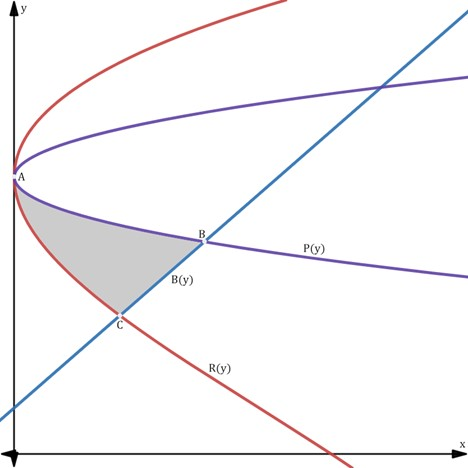
\includegraphics[scale=1]{Question 6 - Graph.jpg}\\
\textit{
    \textbf{Answers by Accurate drawings or graphical methods are not accepted.}\\
    The graphs are plotting y against x. Point A is a common stationary point of\\
    R(y) and P(y). B(y) passes through the points \(D(10 , 2)\) and \(E(1 , \frac{1}{2})\).\\
    \(P(y) = 33(y - 2)^2\) , \(B(y) = R''(y)\)\\
    Degree of polynomial R(y) is 3.
}

    \newpage

\textit{Find the shaded area.\\*
        \textbf{Leave your answers in exact values,} in the form \(a + b\sqrt{339}\) , where \(a, b\in\mathbb{Q}\)
} \qnmark{20}

%%%%%%%%%%%%%%%%%%
%%%%%Solution%%%%%
%%%%%%%%%%%%%%%%%%

%\newpage \ \newpage \ \newpage \ \newpage

%\begin{comment}

%%%%%Showing that B(y) is linear%%%%%
\begin{gather*}
    Degree \; of \; R(y) \; is \; 3 \implies Degree \; of \; B(y) \; is \; 1, \; therefore \; B(y) \; is \; a \; linear \; function
\end{gather*}

%%%%%Finding B(y)%%%%%
\textit{Finding the Equation of B(y)}
\begin{align*}
    \displaystyle   y-2 &= \frac{1}{6}(x-10) \\
    \displaystyle 6y-12 &= x-10 \\
    \displaystyle     x &= 6y-2 \\
    \displaystyle \therefore B(y) &= 6y-2 \onemark \\
\end{align*}

%%%%%Finding R(y) & Point A%%%%%
\textit{Finding the coordinates of point A}
\begin{equation*}
    \displaystyle P'(y) = 66(y-2)
\end{equation*}
\textit{When P(y) = 0}
\begin{align*}
    66(y-2) &= 0 \\
    \therefore y &= 2 \onemark
\end{align*}
\textit{Sub y = 2 into P(y)}
\begin{align*}
    \therefore x &= 33(2-2)^{2}\\
                &= 0 \\
    \implies  A &= (0 , 2) \onemark
\end{align*}

\textit{Finding the equation of R(y)}\\
\textit{Since B(y) = R''(y)}
\begin{align*} %% Finding R'(y)
    \displaystyle R'(y) &= \int{B(y)} \; dy\\
    \displaystyle       &= 3y^{2}-2y+c_{1} , where \; c_{1}\in\mathbb{R} \onemark\\
\end{align*}
\textit{Point A is a stationary point of R(y)\(\implies R'(2) = 0\)}
\begin{align*} %% Finding c_1
    3(2)^{2}-2(2)+c_{1} &= 0 \\
                  c_{1} &= -8 \onemark \\
    \therefore    R'(y) &= 3y^{2}-2y-8
\end{align*}

\newpage

\begin{align*} %% Integrating R'(y)
    R(y) &= \int{R'(y)} \; dy \\
         &= y^{3}+y^{2}-8y+c_{2} , where \; c_{2}\in\mathbb{R} \onemark
\end{align*}
\textit{When x = 0, y = 2,}
\begin{align*}
                  R(2) &= 0 \\
    2^{3}-2{2}-8+c_{2} &= 0 \\
    \therefore  c_{2} &= 12 \onemark \\
    \implies R(y) &= y^{3}-y^{2}-8+12 \\
\end{align*}

%%%%%Finding Points B & C%%%%%
\textit{Given that Point C is an intercept of R(y) and B(y)}
\begin{align*} %% Rewriting R(y) =B(y)
    \displaystyle               R(y) &= B(y) \\
    \displaystyle  y^{3}-y^{2}-8y+12 &= 6y-2 \\
    \displaystyle y^{3}-y^{2}-14y+14 &= 0 \onemark
\end{align*}
\begin{align*} %% Solving the equation
    \displaystyle Let \; f(x) &= y^{3}-y^{2}-14y+14 \\
    \displaystyle f(1) &= 0
\end{align*}
\begin{gather*}
    \displaystyle \therefore (y-1) \; is \; a \; factor \; of \; f(x) \onemark
\end{gather*}
\begin{align*} %% Finding the y-coordinate of C
     f(x) &= (y-1)(y^{2}-14) \\
          &= 0 \\
    \\
    y^{2} &= 14 \\
        y &= \pm\sqrt{14} \\
    \therefore y &= 1 \; or \pm\sqrt{14}
\end{align*}
\begin{gather*}
    Rej. \; y = \pm\sqrt{14} \\
        \implies y = 1 \onemark \\
\end{gather*}
\begin{align*} %% Finding the x-coordinate of C
    Sub. \; y &= 1 \; into \; B(y), \\
    B(1) &= 6(1)-2 \\
         &= 4 \\
    \therefore C &= (4,1) \onemark
\end{align*}

\newpage

%%%%%Finding Point B%%%%%
\textit{Given that Point B is an intercept of P(y) and B(y)}
\begin{align*} %% Rewriting the Equation
    \displaystyle 6y-2 &= 33(y-2)^{2} \onemark \\
    \displaystyle      &= 33y^{2}-132y+132
\end{align*}
\begin{equation*}
    \displaystyle 33y^{2}-138y+134 = 0 \\
\end{equation*}
\begin{align*} %% Finding the values of y
    y &= \frac{138\pm\sqrt{(-138)^{2}-4(33)(134)}}{2(33)} \\
      &= \frac{138\pm\sqrt{1356}}{2(33)} \\
      &= \frac{69\pm\sqrt{339}}{33} \onemark
\end{align*}
\textit{Reject $\displaystyle y = \frac{69+\sqrt{339}}{33}$, $\displaystyle \therefore y = \frac{69-\sqrt{339}}{33}$} \\
\\\\
\textit{Sub $\displaystyle y = \frac{69-\sqrt{339}}{33}$ into B(y)}
\begin{align*} %% Finding Point B
    \displaystyle B\left(\frac{69-\sqrt{339}}{33}\right) &= 6\left(\frac{69-\sqrt{399}}{33}\right)-2 \\
    \displaystyle                                        &= \frac{2\left(69-\sqrt{339}\right)-22}{11} \\
    \displaystyle                                        &= \frac{116-2\sqrt{339}}{11}
\end{align*}
\begin{equation*}
    \displaystyle \therefore B = \left(\frac{116-2\sqrt{339}}{11},\frac{69-\sqrt{339}}{33}\right) \onemark \\
\end{equation*}

\newpage

%%%%%Finding the shaded area%%%%%
\textit{Let S be the shaded area and \(\displaystyle \alpha = \frac{69-\sqrt{339}}{33}\)}
\begin{align*}
    \displaystyle S &= \int_{\alpha}^{2} P(y) \, dy + \frac{1}{2}\left(\frac{69-\sqrt{339}}{33}-1\right)\left(\frac{116-2\sqrt{339}}{11}+4\right) - \int_{1}^{2} R(y) \, dy \\
    \displaystyle   &= \int_{\alpha}^{2} 33(y-2)^{2} \, dy + \frac{1}{2}\left(\frac{69-\sqrt{339}}{33}-1\right)\left(\frac{116-2\sqrt{339}}{11}+4\right) - \int_{1}^{2} y^{3}-y^{2}-8y+12 \, dy \onemark \\
    \displaystyle   &= \left[11(y-2)^3\right]_{a}^{2} + \frac{1}{2}\left(\frac{36-\sqrt{339}}{33}\right)\left(\frac{160-2\sqrt{339}}{11}+4\right) - \left[\frac{y^{4}}{4}-\frac{y^{3}}{3}-4y^{2}+12y\right]_{1}^{2} \onemark \\
    \displaystyle   &= -11\left(\frac{69-\sqrt{339}}{33}-2\right)^{3} + \frac{\left(36-\sqrt{339}\right)\left(160-2\sqrt{339}\right)}{726} \\
    \displaystyle   &  -\left(\frac{2^{4}}{4}-\frac{2^{3}}{3}-4(2)^{2}+12(2)-\left(\frac{1}{4}-\frac{1}{3}-4+12\right)\right) \onemark \\
    \displaystyle   &= -11\left(\frac{3-\sqrt{339}}{33}\right)^{3}+\frac{6438-232\sqrt{339}}{726}-\frac{17}{12} \\
    \displaystyle   &= \frac{-44\left(3078-366\sqrt{339}\right)+99\left(12029-464\sqrt{339}\right)}{143748} \\
    \displaystyle   &= \frac{1055439-62040\sqrt{339}}{143748}  \\
    \displaystyle   &= \frac{10661}{1452}-\frac{470}{1089}\sqrt{339} \\
    \\
    \displaystyle   &  \therefore the \; shaded \; area \; is \left(\frac{10661}{1452}-\frac{470}{1089}\sqrt{339}\right) \, u^{2} \onemark
\end{align*}

%\end{comment}
 \newpage
  \item \textbf{\hypertarget{P7}{[\,Suggested Time: 20 mins \textbar \, Total Marks: 10 \textbar \, Challenging\,]}}\\
%%%%%Question i, Proving the parallel eff. resistance equation%%%%%
\\
\textbf{Circuit Theory} \\
\textit{The workings of a parallel circuit can be explained with a water tank, where the water \\
        tank is like a battery in the circuit, current \(I\) is the water flowing in the pipes, \\
        voltage \(V\) can be seen as the pressure which the water experiences at a \\
        certain point and resistance \(R\) is a measure of how much pressure is \\
        needed to move a certain quantity of water from a point to another}
\begin{center}
    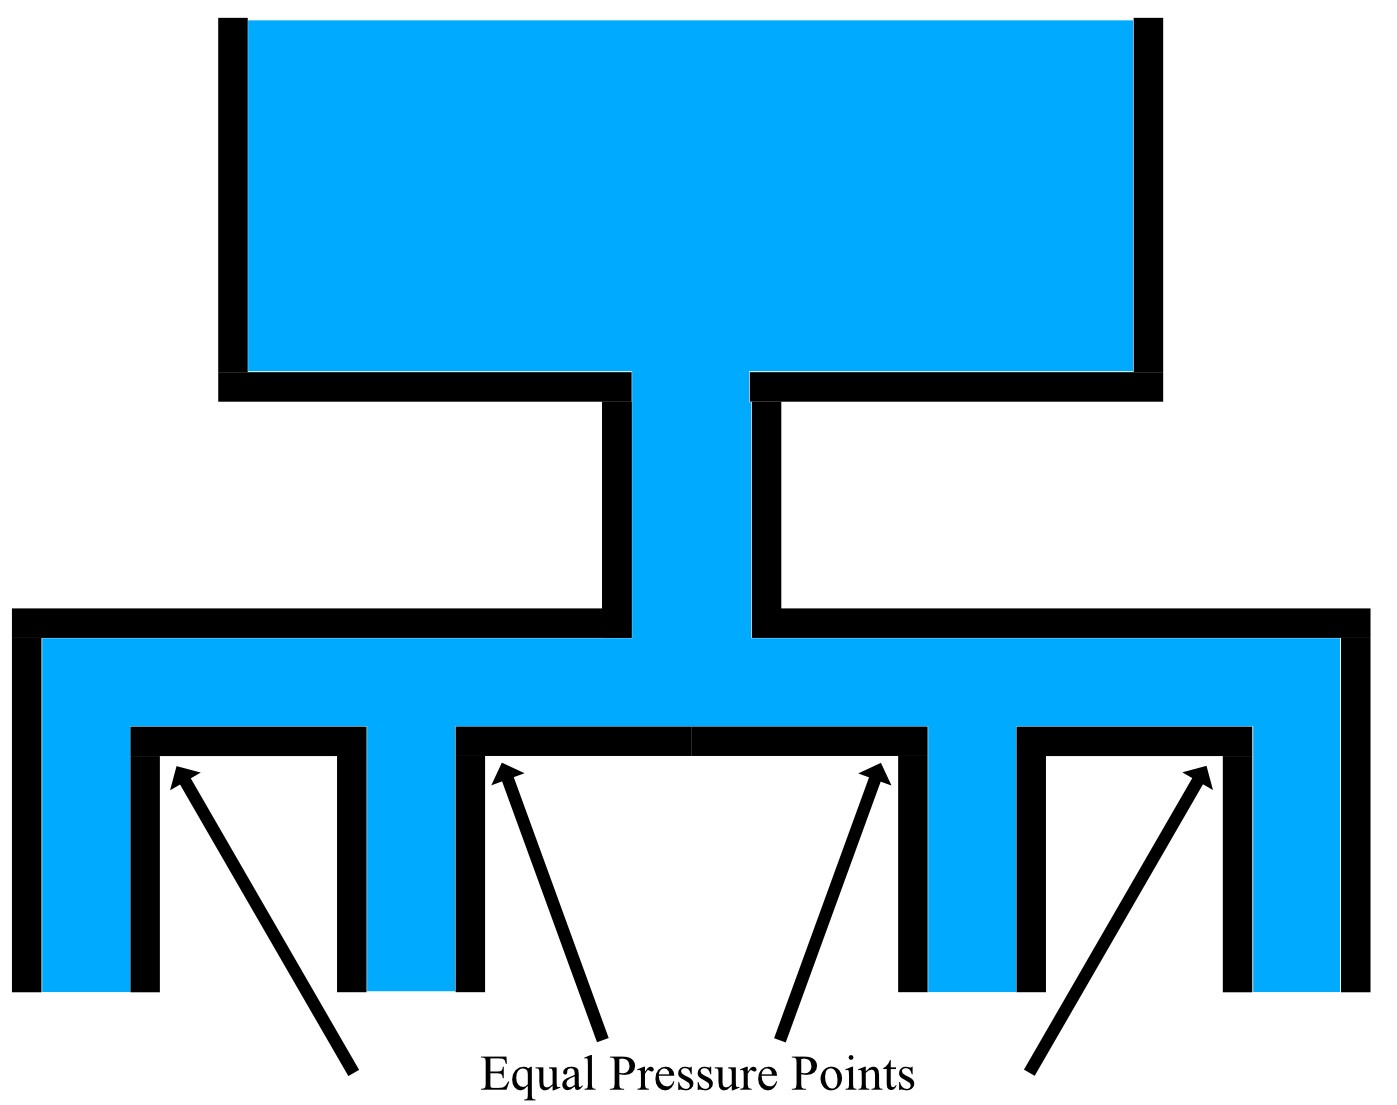
\includegraphics[scale=0.7]{Question 7i - Water Tank.jpg}
\end{center}
\textit{In the diagram shown above, it is known that the pressure at all 4 points which the arrows \\
        are pointing at are equivalent, and the total volume of water that flows out of the pipes \\
        is equal to the volume of water that flows into the  pipes from the water tank. \\
        \\
        It is also given that ohmic conductors follow ohm's law, \(V = IR\) \\
}

\begin{center}
    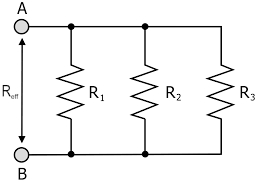
\includegraphics[scale=1.2]{Question 7i - Circuit Diagram.jpg}
\end{center}

\newpage

\textit{
    \textbf{(i)} Using the information given above, deduce the effective resistance, \(R_{eff}\), in \\
    \hspace*{20pt} the circuit shown above, and consequently, find an expression for a parallel \\
    \hspace*{20pt} circuit with n resistors. \textbf{Leave your answers in terms of V,I and R}
} \qnmark{5} \\

%%%%%%%%%%%%%%%%%%
%%%%%Solution%%%%%
%%%%%%%%%%%%%%%%%%

%\begin{comment}

%%%%%Electricity laws in a parallel circuit%%%%%
\textit{From the question, we can deduce that the
}
\begin{gather*}
    Total \; current, \; I_{T}, \; in \; the \; circuit \; is \; I_{T} = I_{1}+I_{2}+I_{3} \\
    Total \; voltage, \; V_{T}, \; across \; the \; circuit \; is \; V_{T} = V_{1} = V_{2} = V_{3} \onemark \\
\end{gather*}
\textit{By Ohm's law, we can see that}
\begin{equation*}
    \displaystyle I_{1} = \frac{V_{1}}{R_{1}}, I_{2} = \frac{V_{2}}{R_{2}}, I_{3} = \frac{V_{3}}{R_{3}} \onemark \\
\end{equation*}

%%%%%Proving R_{eff} for 3 resistors%%%%%
\textit{Using the total current and voltage equations that we had deduced,}
\begin{align*}
    \displaystyle I_{T} &= \frac{V_{1}}{R_{1}} + \frac{V_{2}}{R_{2}} + \frac{V_{3}}{R_{3}} \\
    \displaystyle       &= \frac{V_{T}}{R_{1}} + \frac{V_{T}}{R_{2}} + \frac{V_{T}}{R_{3}} \\
    \displaystyle       &= V_{T}\left(\frac{1}{R_{1}} + \frac{1}{R_{2}} + \frac{1}{R_{3}}\right) \onemark \\
\end{align*}
\begin{align*}
    \displaystyle \therefore R_{eff} &= \frac{V_{T}}{I_{T}} \\
    \displaystyle                    &= \frac{V_{T}}{V_{T}\left(\displaystyle \frac{1}{R_{1}} + \frac{1}{R_{2}} + \frac{1}{R_{3}}\right)} \\
    \displaystyle                    &= \frac{1}{\left(\displaystyle \frac{1}{R_{1}} + \frac{1}{R_{2}} + \frac{1}{R_{3}}\right)} \\
    \displaystyle                    &= \left(\displaystyle \frac{1}{R_{1}} + \frac{1}{R_{2}} + \frac{1}{R_{3}}\right)^{-1} \tag*{\qedsymbol} \\ \onemark \\
\end{align*}

%%%%%Proving the equation in the question%%%%%
\textit{Since we know that \(V_{T} = V_{1} = V_{2} = V_{3} = \cdots\), \\
        and that \(V_{T}\) would be eliminated in the expression, \\
        \\
        Following the same process, we can generalize the expression for n resistors as
}
\begin{gather*}
    \displaystyle R_{eff} = \left(\frac{1}{R_{1}}+\frac{1}{R_{2}}+\frac{1}{R_{3}}+\cdots+\frac{1}{R_{n}}\right)^{-1} \tag*{\qedsymbol} \\ \onemark
\end{gather*}

%\end{comment}

\newpage \ \newpage %%Don't Comment This

%%%%%Question iia, finding the eff. resistance of a parallel resistor system%%%%%
\begin{center}
    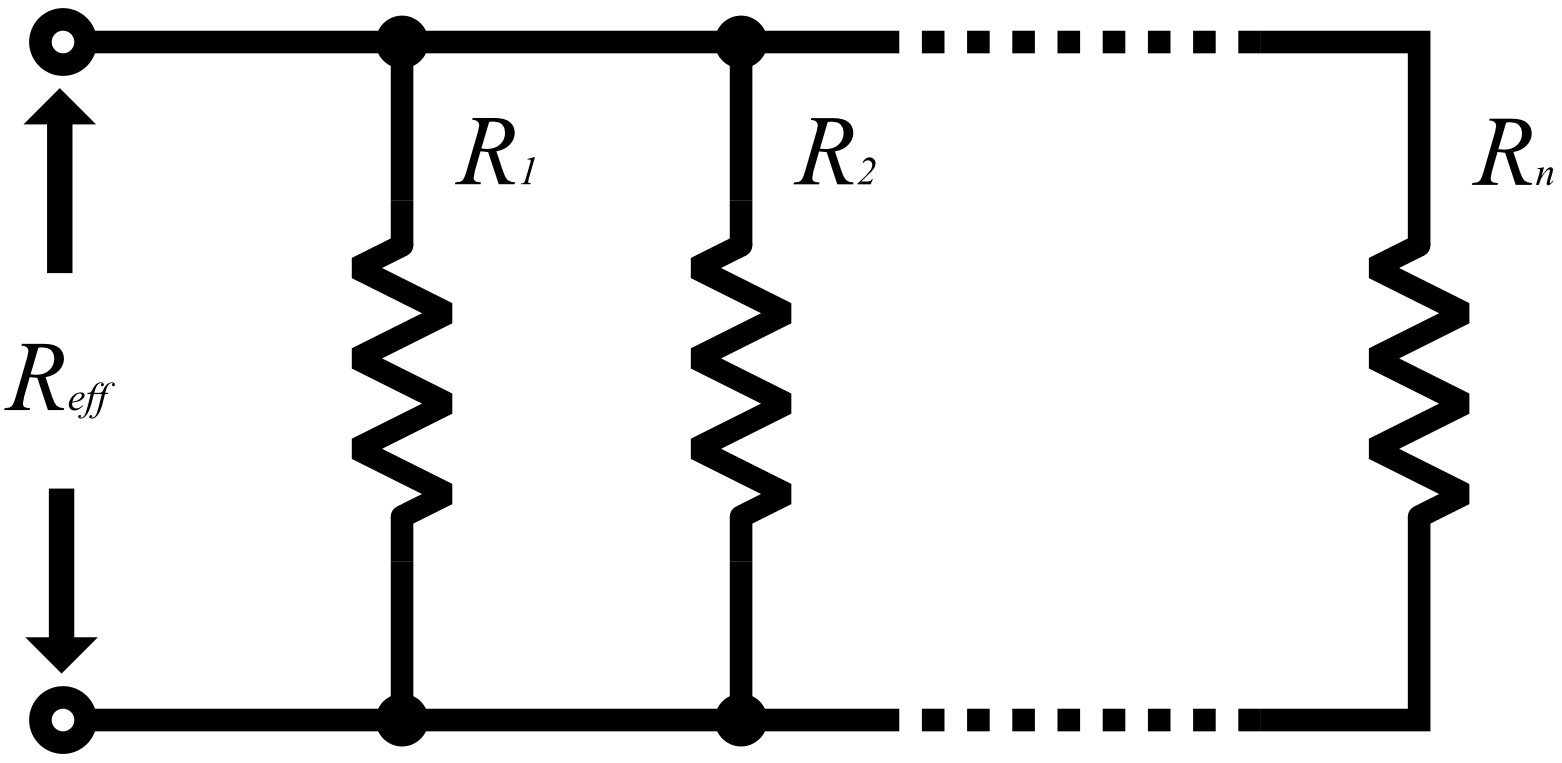
\includegraphics[scale=0.25]{Question 7iia - Circuit Diagram.jpg}
\end{center}
\textit{\textbf{(ii)(a)} Hence, using (i) or otherwise, find the effective resistance of the circuit shown above. \\
        \hspace*{35pt} Where \(R_{1} = \sqrt{1}+\sqrt{2}, R_{2} = \sqrt{2}+\sqrt{3}, R_{3} = \sqrt{3}+\sqrt{4} \; \cdots\) \\
        \hspace*{35pt} \textbf{Leave your answers in exact values}, and in terms of n.
} \qnmark{4} \\

%%%%%%%%%%%%%%%%%%
%%%%%Solution%%%%%
%%%%%%%%%%%%%%%%%%

%\begin{comment}

%%%%%Finding the effective resistance%%%%%
\textit{We can see that the resistance of the resistors follow a series with a general term of}
\begin{equation*}
    \displaystyle R_{n} = \sqrt{n}+\sqrt{n+1} \onemark \\
\end{equation*}

\begin{align*}
    \displaystyle \therefore R_{eff} &= \left(\frac{1}{\sqrt{1}+\sqrt{2}}+\frac{1}{\sqrt{2}+\sqrt{3}}+\frac{1}{\sqrt{3}+\sqrt{4}}+\cdots+\frac{1}{\sqrt{n}+\sqrt{n+1}}\right)^{-1} \onemark \\
    \displaystyle                    &= \left(\frac{\sqrt{1}-\sqrt{2}}{1-2}+\frac{\sqrt{2}-\sqrt{3}}{2-3}+\frac{\sqrt{3}-\sqrt{4}}{3-4}+\cdots+\frac{\sqrt{n}-\sqrt{n+1}}{n-n-1}\right)^{-1} \onemark \\
    \displaystyle                    &= \left(\left(\sqrt{2}-\sqrt{1}\right)+\left(\sqrt{3}-\sqrt{2}\right)+\left(\sqrt{4}-\sqrt{3}\right)+\cdots+\left(\sqrt{n+1}-\sqrt{n}\right)\right)^{-1} \\
    \displaystyle                    &= \left(\sqrt{n+1}-1\right)^{-1} \\
    \displaystyle                    &= \frac{1}{\sqrt{n+1}-1} \onemark
\end{align*}

\textit{The effective resistance of the circuit is \(\displaystyle \frac{1}{\sqrt{n+1}-1}\), \\ \
        where n is the number of resistors
}

%\end{comment}

\newpage \ \newpage %%Don't Comment This

%%%%%Question iib, proving if this is converging series%%%%%
\textit{\textbf{(ii)(b)} Explain, with relevant workings, if the effective resistance of the circuit \\
        \hspace*{40pt} will approach a unique value as more resistors are added into the circuit.
} \qnmark{1} \\

%%%%%%%%%%%%%%%%%%
%%%%%Solution%%%%%
%%%%%%%%%%%%%%%%%%

%\begin{comment}

\textit{from (ii)(a), \(\displaystyle R_{eff} = \frac{1}{\sqrt{n+1}-1}\)} \\
\begin{align*}
    \displaystyle As \; n \rightarrow \infty, \; \sqrt{n+1}-1 &\rightarrow \infty \\
    \displaystyle                      \frac{1}{\sqrt{n+1}-1} &\rightarrow 0 \\
    \displaystyle                          \therefore R_{eff} &\rightarrow 0 \onemark
\end{align*}
\textit{Yes, \(R_{eff}\) approaches the value 0 as more resistors are added into the circuit}


%\end{comment} \newpage
  \item \textbf{\hypertarget{P8}{[\,Suggested Time: 20 mins \textbar \, Total Marks: 10 \textbar \, Challenging\,]}} \\\\
\textbf{Fermat's Principle of Least Time} \\
\textit{Fermat's Principle of Least Time states that out of all neighbouring paths available, \\
        light travels between two points along the path that requires the least time.\\
        \\
        Consider a light ray from a source which strikes a mirror and is reflected. Let A be \\
        a point on the ray before it strikes the mirror and B be the point on the ray after \\
        reflection. v m/s  is the speed of light. \\
        \\
        A coordinate system is placed in a plane such that the x-axis runs along the mirror's \\
        surface and the point A lies on the y-axis.
        \\
}
\begin{center}
    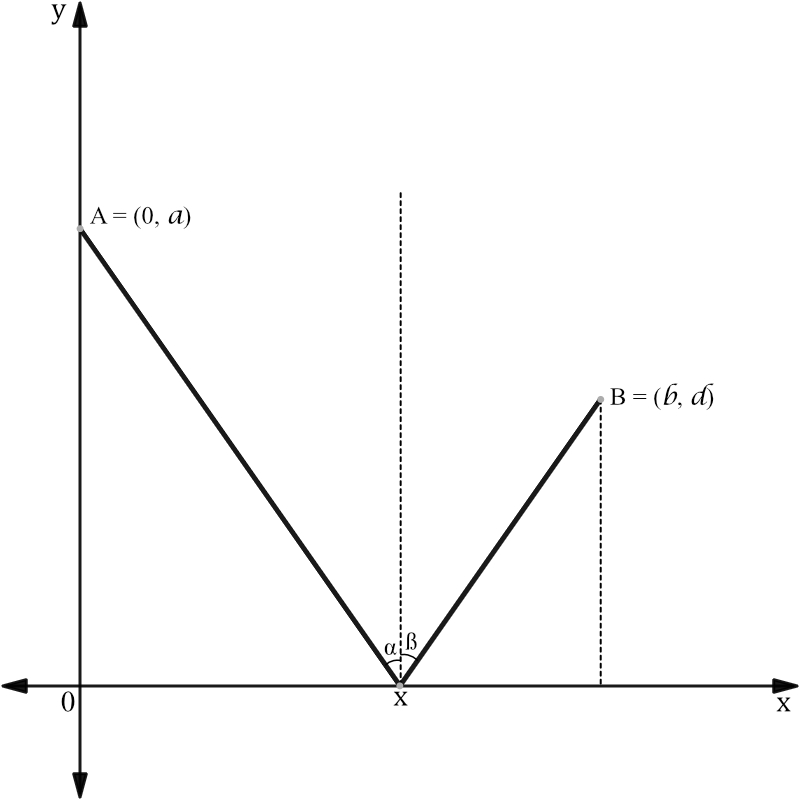
\includegraphics[scale=0.4]{Problem 8 - Reference Diagram.jpg}
\end{center}

\newpage

\textit{Prove that the angle of incidence \(\alpha\) is equal to the angle of reflection \(\beta\). \\
        (Proof that T is minimum is not required)} \qnmark{10}

%%%%%%%%%%%%%%%%%%
%%%%%Solution%%%%%
%%%%%%%%%%%%%%%%%%

%\begin{comment}
    \textit{\\ Note that \(\displaystyle \tan{\alpha} = \frac{x}{a}\) and \(\displaystyle \tan{\beta} = \frac{b-x}{d}\)}

    %%%%%Finding the function T%%%%%
    \begin{align*}
        \displaystyle T &= \frac{Distance}{Speed} \\
        \displaystyle   &= \frac{|Ax|}{v}+\frac{|Bx|}{v} \onemark \\
        \displaystyle   &= \frac{1}{v}\sqrt{a^{2}+x^{2}} + \frac{1}{v}\sqrt{d^{2}+(b-x)^{2}} \onemark \\
        \displaystyle   &= \frac{1}{v}\left(\sqrt{a^{2}+x^{2}}+\sqrt{d^{2}+(b-x)^{2}}\right)
    \end{align*}
    
    %%%%%Differentiating T w.r.t. x%%%%%
    \begin{align*}
        \displaystyle \therefore \frac{dT}{dx} &= \frac{1}{v}\left(\frac{x}{\sqrt{a^{2}+x^{2}}}-\frac{b-x}{\sqrt{d^{2}+(b-x)^2}}\right) \twomark \\
        \displaystyle                          &= \left(\frac{x\sqrt{d^{2}+(b-x)^2}-(b-x)\sqrt{a^{2}+x^{2}}}{v\sqrt{\left(a^{2}+x^{2}\right)\left(d^{2}+(b-x)^{2}\right)}}\right) \onemark \\
    \end{align*}

    %%%%%Finding the min. value of T%%%%%
    \textit{For minimum T,}
    \begin{align*}
        \displaystyle \frac{dT}{dx} &= 0 \\
        \displaystyle \frac{x\sqrt{d^{2}+(b-x)^2}-(b-x)\sqrt{a^{2}+x^{2}}}{v\sqrt{\left(a^{2}+x^{2}\right)\left(d^{2}+(b-x)^{2}\right)}} &= 0 \onemark \\
        \displaystyle                                                                      x\sqrt{d^{2}+(b-x)^2}-(b-x)\sqrt{a^{2}+x^{2}} &= 0 \onemark \\
        \displaystyle                                                                                              x\sqrt{d^{2}+(b-x)^2} &= (b-x)\sqrt{a^{2}+x^{2}} \\
        \displaystyle                                                                                    x^{2}\left(d^{2}+(b-x)^2\right) &= (b-x)^{2}\left(a^{2}+x^{2}\right) \onemark \\
        \displaystyle                                                            x^{2}d^{2}+x^{2}(b-x)^{2}-a^{2}(b-x)^{2}-x^{2}(b-x)^{2} &= 0 \\
        \displaystyle                                                                                          x^{2}d^{2}-a^{2}(b-x)^{2} &= 0 \\
        \displaystyle                                                                                                         x^{2}d^{2} &= a^{2}(b-x)^{2} \\
        \displaystyle                                                                                                                 xd &= a(b-x) \\
        \displaystyle                                                                                                        \frac{x}{a} &= \frac{b-x}{d} \\
        \displaystyle                                                                                                       \tan{\alpha} &= \tan{\beta} \onemark
    \end{align*}
    \begin{gather*}
        Since \; both \; \alpha \;\&\; \beta \; are \; acute, \\
        \implies \alpha = \beta \tag*{\qedsymbol} \\ \onemark
    \end{gather*}

%\end{comment}

\newpage \ \newpage \newpage
  \item \textbf{\hypertarget{P9}{[\,Suggested Time: 25 mins \textbar \, Total Marks: 12 \textbar \, Challenging\,]}}\\
    A soft drink company wants to design a 500ml soda can using the least amount of \\
    material for their new Moon Shine soda. Assume that the soda can is a perfect \\
    cylinder. Using the information given below, find the cheapest material cost to \\
    produce 1000 cans. \textbf{Leave your answers in USD}  \qnmark{12} \\

%%%%%Information List%%%%%
\begin{center}
    \begin{tabularx}{0.65\textwidth} {
        | >{\centering\arraybackslash}X
        | >{\centering\arraybackslash}X| }
        \hline
        \multicolumn{2}{|c|}{\textbf{Information List}} \\
        \hline
        \textbf{Price of Aluminium} & \(2515 \; USD/Metric \; Tonne\) \\
        \hline
        \textbf{Density of Aluminium} & \(2.7g/cm^{3}\) \\
        \hline
        \textbf{1 Atmosphere (Pressure)} & 101325 Pa \\
        \hline
        \textbf{Room Temperature} & \(T_{c} = 28^{\circ}c\) \\
        \hline
        \textbf{Temperature (Kelvin)} & \(T_{k} = T_{c}+273\) K \\
        \hline
        \textbf{Gas Constant (R)} & \(R = 8.314\,m^{3}\,Pa/mol\,K\) \\
        \hline
    \end{tabularx}
    \\
    \vspace*{25pt}
    \begin{tabularx}{0.65\textwidth} {
        | >{\centering\arraybackslash}X| }
        \hline
        \textbf{Ideal Gas Law} \\
        \hline
        \textit{\textbf{PV = nRT} }\\*
        \(P - Pressure\) \\*
        \(V - Volume\) \\*
        \(n - Amount\;of\;Substance\) \\*
        \(R - Gas\;Constant\) \\*
        \(T - Temperature\) \\
        \hline
    \end{tabularx}
\end{center}

\vspace*{25pt}

    The Soda can is able to tolerate up to 5 atm of pressure, and has a uniform thickness \\
    of \(0.01\;cm\). The soda releases up to \(\displaystyle \frac{x}{10}\;cm^{3}\) of gas for every \(x\;ml\) of soda under room \\
    temperature and pressure.

\newpage

%%%%%%%%%%%%%%%%%%
%%%%%Solution%%%%%
%%%%%%%%%%%%%%%%%%

%\newpage \ \newpage \ \newpage

%\begin{comment}

%%%%%Formula for Surface area and Volume of Can%%%%%
Let \(S_{c}\;\&\;V_{c}\) be the total surface area and volume of the can respectively

\begin{align*}
    \displaystyle S_{c} &= 2 \pi rh+2\pi r^{2} \\
    \displaystyle V_{c} &= \pi r^{2}h
\end{align*}

%%%%%Finding the Volume of gas in the can at 5Pa (Max Pressure)%%%%%
    Room temperature and pressure \(\implies P = 1\;atm,\;T_{c} = 28^{\circ}c\) \\\\
    Thus, using the Ideal gas law, the number of moles of gas is
\begin{align*}
    \displaystyle n &= \frac{PV}{RT} \\
    \displaystyle   &= \frac{101325\left(\displaystyle \frac{50}{100^{3}}\right)}{8.314(273+28)} \\
    \displaystyle   &= 2.0245 \times 10^{-3} \wrkonemark \\
\end{align*}

    Since the max pressure that the can is able to handle is 5 atm, \\
    min volume taken up by gas is,
\begin{align*}
    \displaystyle V &= \frac{nRT}{P} \\
    \displaystyle   &= \frac{2.0245 \times 10^{-3}(8.314\times(273+28))}{5(101325)} \\
    \displaystyle   &= 1\times 10^{-5}\;m^{3} \\
    \displaystyle   &= 10\;cm^{3} \wrkonemark \\
\end{align*}
\textit{Thus, $V_{c} = 500 + 10 = 510 cm^{3}$}
\begin{align*}
    \displaystyle 510 &= \pi r^{2}h \\
    \displaystyle   h &= \frac{510}{\pi r^{2}} \wrkonemark
\end{align*}

%%%%%Finding the radius that gives the min. suf. area%%%%%
\begin{align*}
    \displaystyle  \therefore S_{c} &= 2\pi r\left(\frac{510}{\pi r^{2}}\right) + 2\pi r^{2} \\
    \displaystyle                   &= \frac{1020}{r} + 2\pi r^{2} \\
    \displaystyle \frac{dS_{c}}{dr} &= 4\pi r - \frac{1020}{r^{2}} \wrkonemark
\end{align*}

\newpage

When \(\displaystyle \frac{dS_{c}}{dr} = 0\)
\begin{align*}
    \displaystyle    4\pi r - \frac{1020}{r^{2}} &= 0 \wrkonemark \\
    \displaystyle \frac{4\pi r^{3} -1020}{r^{3}} &= 0 \\
    \displaystyle               4\pi r^{3} -1020 &= 0 \\
    \displaystyle \therefore               r^{3} &= \frac{1020}{4\pi} \\
    \displaystyle                              r &= \sqrt[3]{\frac{255}{\pi}} \approx 4.3298\;cm \wrkonemark
\end{align*}
\begin{align*} %%2nd Derivative Test
    \displaystyle                                                         \frac{d^{2}S_{c}}{dr^{2}} &= 4\pi + \frac{2040}{r^{3}} \\
    \displaystyle \left.\frac{d^{2}S_{c}}{dr^{2}}\right|_{\textstyle r = \sqrt[3]{\frac{300}{\pi}}} &= 4\pi + \frac{2040\pi}{255} \\
    \displaystyle                                                                                   &> 0 \wrkonemark
\end{align*}
\(\therefore \displaystyle r = \sqrt[3]{\frac{255}{\pi}}\) gives a min. amount of aluminium used

%%%%%Mass of aluminium required to make 1000 cans%%%%%
\begin{align*}
    \displaystyle V_{alu} &= \pi \left(0.01+\sqrt[3]{\frac{255}{\pi}}\right)^{2}\left(\frac{510}{\pi \left(\textstyle \sqrt[3]{\frac{255}{\pi}}\right)^{2}} + 0.02\right) - 510 \\
    \displaystyle         &\approx 3.5419\;cm^{2} \wrkonemark \\\\
\end{align*}
\begin{align*}
    \text{Mass of 1 Can} &= 3.5419(2.7) \\
                         &= 9.56313g \wrkonemark \\
    \text{Mass of 1k Cans}  &= 9.56313(1000) \\
                            &= 9563.13g \\
                            &\approx 9.5631kg \wrkonemark
\end{align*}

%%%%%Least material cost to produce 1000 cans%%%%%
\begin{align*}
    \displaystyle \text{Price of Aluminium in kg} &= \frac{2515}{1000} \\
                                                  &= 2.515 \; USD/kg \wrkonemark
\end{align*}
\begin{align*}
    \therefore \text{Material Cost to produce 1000 Cans} &= 9.5631(2.515) \\
                                                         &\approx 24.05 \; USD \ansonemark
\end{align*}
%\end{comment}

 \newpage
  \item \textbf{\hypertarget{P10}{[\,Suggested Time: N.A. \textbar \, Total Marks: N.A. \textbar \, Schadenfreude\,]}} \\
\textit{Given that if x satisfies \(\displaystyle x^{n}+a_{n-1}x^{n-1}+\cdots+a_{0} = 0\) for some integers \(a_{n-1},\cdots, a_{0}\), \\
        then x is irrational unless x is an integer. \\
        Prove that \(\sqrt{2}+\sqrt[3]{2}\) is irrational. \\
}

%%%%%%%%%%%%%%%%%%
%%%%%Solution%%%%%
%%%%%%%%%%%%%%%%%%

%\begin{comment}

    \textit{Let \(\displaystyle x = \sqrt{2}+\sqrt[3]{2}\). Now we see that:}
    \begin{align*}
        \displaystyle       \left(x-\sqrt{2}\right)^{3} &= 2 \\
        \displaystyle   x^{3}\sqrt{2}x^{2}+6x+2\sqrt{2} &= 2 \\
        \displaystyle                        x^{3}+6x-2 &= \sqrt{2}\left(3x^{2}-2\right) \\
        \displaystyle       \left(x^{3}+6x-2\right)^{2} &= 2\left(3x^{2}-2\right)^{2} \\
        \displaystyle x^{6}-6x^{4}-4x^{3}+36x^{2}-24x+4 &= 2(9x^{4}+12x^{2}+4) \\
        \displaystyle x^{6}-6x^{4}-4x^{3}+12x^{2}-24x-4 &= 0 \\
    \end{align*}
    \textit{Therefore, we have found a monic polynomial with integer coefficients which has \\
            \(\displaystyle \sqrt{2}+\sqrt[3]{2}\) as its root, meaning by the equation given, \(\displaystyle \sqrt{2}+\sqrt[3]{2}\) must either be an \\
            integer or irrational number. It is trivial that \(\displaystyle \sqrt{2}+\sqrt[3]{2}\) is not an integer, hence \\
            it has to be an irrational number.
    }

%\end{comment}

\newpage \ \newpage
\end{enumerate}

\end{document}